\chapter{DISCRETIZAÇÃO} \label{cap:disc}
\vspace{-2cm}
A estimação de densidade via \ac{KDE} de uma série de medidas contínuas, por razões computacionais, é geralmente representado na forma discreta. Consequentemente, estimações diretas acontecem apenas para valores discretizados \cite{jones1989discretized} e interpolação é usado para solucionar qualquer outro valor que possa vir fora durante as mediações. Este processo insere erros de estimação os quais podem ser minimizados incrementando o número de pontos a serem estimados, buscando um equilíbrio entre otimização computacional e performance de estimação.

Vários autores seguem a mesma abordagem, como em \cite{jones1989discretized}, explorando os diferentes aspectos do processo de discretização e propondo novos métodos no intuito de minimizar as adversidades relatadas. Por exemplo, em \cite{fayyad1993multi} o método bem conhecido Ent-MDLP é proposto; em \cite{friedman1996discretizing} é sugerido um algoritmo de discretização baseado em Redes Bayesianas; em \cite{biba2007unsupervised} os autores propõem um método não supervisionado para discretização utilizando-se o \ac{KDE}; também usando o método não supervisionado, os autores de \cite{schmidberger2005unsupervised} apresentam um estudo de discretização aplicado à estimação de densidade baseado em árvore; e em \cite{zhang2007discretization} um algoritmo de aprendizagem de máquina baseado-se no critério de \textit{Gini} foi estudado. 

Estes trabalhos geralmente possuem foco em algoritmos de aprendizagem de máquina ou minimização dos critérios selecionados a fim de otimizar os vários atributos existentes, que como consequência, tendem a ter um alto custo computacional quando submetidos a uma grande quantidade de dados. Além do mais, tais estudos abordam a performance da discretização através do prisma da classificação e alguns como forma de preprocessamento do conjunto de dados.

O método de discretização mais aplicado atualmente é o baseado em espaçamento uniforme entre os pontos estimados. Isso trata de maneira igualitária todas as densidades de região (e. g. a função de densidade nas regiões de baixa probabilidade é discretizada com a mesma resolução das regiões de alta probabilidade) levando a um erro de estimação que tende a não ser uniforme ao longo de todas as regiões de função de densidade de probabilidade.
A figura~\ref{fig:figura1} mostra um exemplo de quando a região de baixa probabilidade é grande devido a eventos fora da curva, neste caso, uma discretização baseada em um espaçamento uniforme  pode colocar um grande número de pontos desnecessários nessa região, fazendo com que, para minimizar o erro de estimação, o número de pontos a ser estimado seja maior a fim de representar bem a região de alta probabilidade. %enquanto regiões de alta probabilidade terão que usar mais pontos a fim de minimizar o erro de estimação.

\begin{figure}[H]
	\centering
	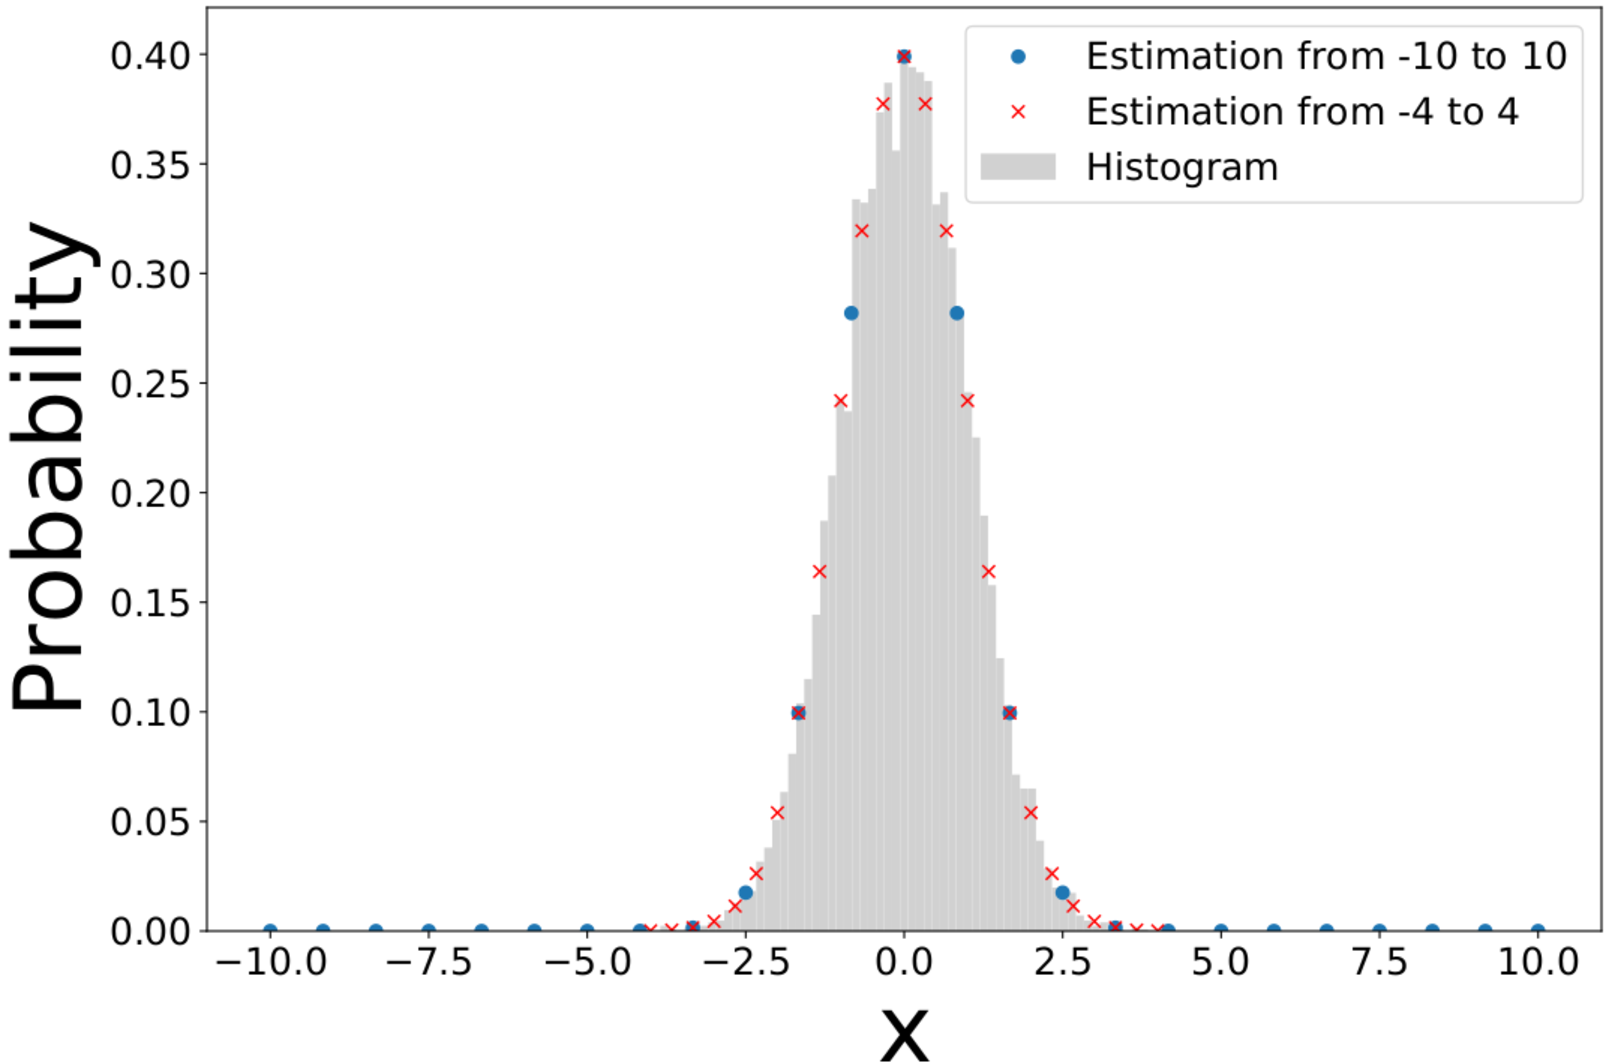
\includegraphics[width=0.6\linewidth]{figuras/linspace2}
	\caption{Caso representativo de estimação de PDF utilizando 25 pontos para dois intervalos diferentes (-4,4) e (-10,10)}
	\label{fig:figura1}
\end{figure}


\section{Métodos de Discretização} \label{cap:metodos}
Para se estudar os efeitos da discretização no processo de estimação de \ac{PDF}, a performance de cinco diferentes métodos serão confrontados, como listados abaixo: 
\begin{itemize}
	\item \textit{Linspace};
	\item \textit{CDFm};
	\item \textit{PDFm};
	\item \textit{iPDF1};
	\item \textit{iPDF2}.
\end{itemize}

Estes cinco métodos serão demostrados a priori  utilizando-se uma distribuição Gaussiana com média $\mu = 0$ e desvio padrão $\sigma = 1$, cuja \ac{PDF} pode ser descrita pela Equação~\eqref{equ:Normal} e ilustrada na Figura~\ref{fig:Gaussiana} com o numero de pontos $N = 25$ para uma melhor visualização.

\begin{equation}
{\displaystyle f_{X}(x;\mu,\sigma) = \frac{1}{\sigma\sqrt{2\pi}}\cdot e^{-\frac{(x-\mu)^2}{2\sigma^2}}}
\label{equ:Normal}
\end{equation}


\begin{figure}[H]
	\centering
	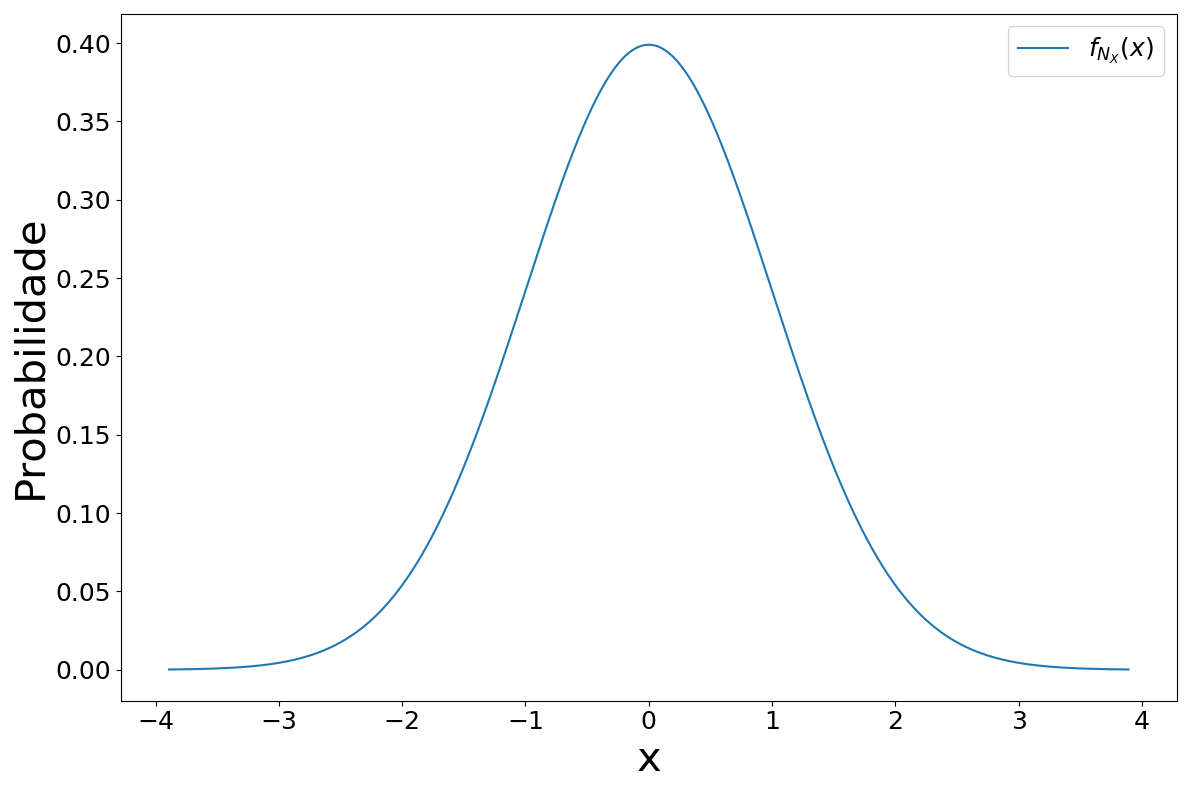
\includegraphics[width=0.6\linewidth]{./figuras/Normal}
	\caption{Ilustração da curva Gaussiana com média $\mu = 0$ e desvio padrão $\sigma = 1$.}
	\label{fig:Gaussiana}
\end{figure}

\subsection{\textit{Linspace}}
O método \textit{Linspace} é caracterizado por amostrar de maneira uniforme a variável aleatória, representada pelo eixo das abscissas de uma \ac{PDF} qualquer. Após, o eixo $ x $ terá \textit{N} pontos igualmente espaçados entre dois valores predefinidos que definem os parâmetros de início e término da distribuição. Este método é o mais utilizado na literatura devido a sua simplicidade. A Figura~\ref{fig:linspace_curve} ilustra o método \textit{Linspace} para a distribuição Normal, limitando o eixo horizontal à uma área de probabilidade de $99,99\%$.


\begin{figure}[H]
	\centering
	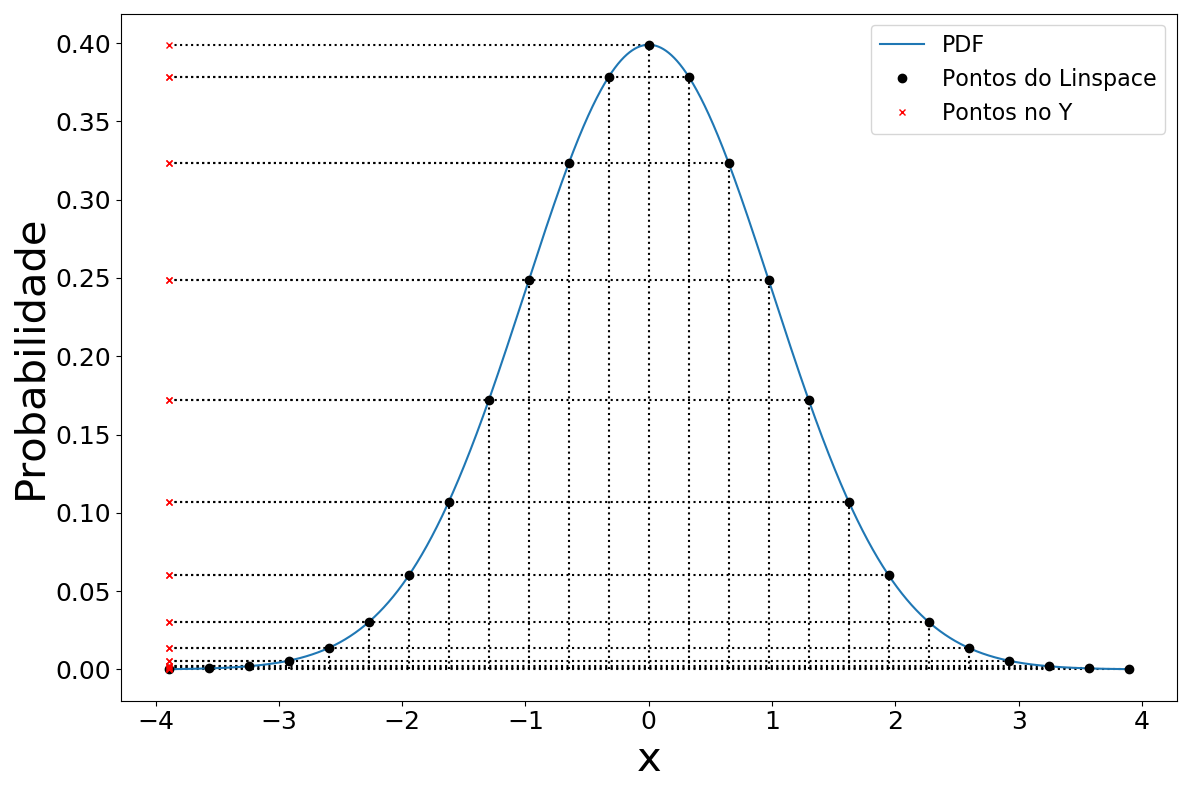
\includegraphics[width=0.7\linewidth]{./figuras/normal_1}
	\caption{Ilustração do método \textit{Linspace} aplicado à uma distribuição normal.}
	\label{fig:linspace_curve}
\end{figure}


\subsection{\textit{CDFm}}
O método denominado nesse trabalho de \ac{CDFm} representa a discretização baseada na \ac{CDF} descrita pela Equação~\eqref{equ:CDF} para uma variável contínua e \eqref{equ:CDF_disc} para o caso de uma variável discreta possuindo valores em $ b $. Para este método, no caso de se ter a função geradora, primeiramente calcula-se a \ac{CDF} da distribuição e então faz-se uma distribuição linear de pontos no eixo $ y $ e encontra-se os seus respectivos valores para o eixo $ x $ fazendo sua função inversa, conforme mostra a Equação~\eqref{equ:cdf_inv} e é ilustado pela Figura~\ref{fig:CDFm_curve}.


%a discretização baseada no espaçamento uniforme é aplicada ao eixo vertical e então os relativos valores horizontais são encontrados refletindo todos os valores, como mostra a Figura~\ref{fig:CDFm_curve} para a distribuição Normal. Note que, quanto maior a probabilidade da \ac{PDF}, maior o número de pontos na sua região.

\begin{equation}
\displaystyle F_X(x) = \int_{-\infty}^{x} f_X(t)dt
\label{equ:CDF}
\end{equation}

\begin{equation}
 {P} (X=b)=F_{X}(b)-\lim _{x\to b^{-}}F_{X}(x)
 \label{equ:CDF_disc}
\end{equation}

\begin{equation}
CDFm(y) = F^{-1}_X(x)
\label{equ:cdf_inv}
\end{equation}

\begin{figure}[H]
	\centering
	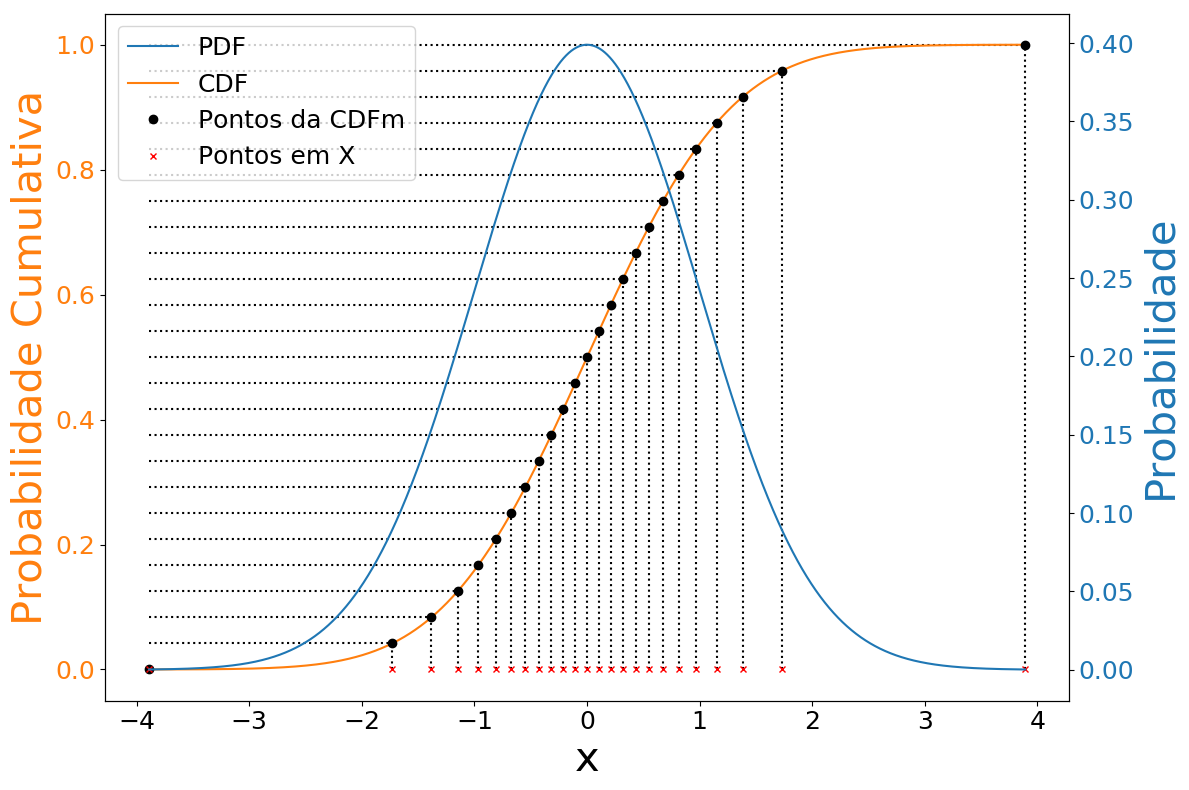
\includegraphics[width=0.6\linewidth]{./figuras/CDFm_normal_1}
	\caption{Ilustração da discretização da distribuição Gaussiana baseada em sua CDF.}
	\label{fig:CDFm_curve}
\end{figure}

É possível notar que, quanto maior a probabilidade da \ac{CDF}, maior o número de pontos em sua região.

\subsection{\textit{PDFm}}
Este método, denominado de \ac{PDFm} também usa a técnica de reflexão aplicada ao método da \textit{CDFm}, mas a função de referência é a própria \ac{PDF}, ao invés da sua \ac{CDF}, com isso, os pontos de intercessão da curva com os valores em $ y $ são calculados. A Figura~\ref{fig:PDFm_curve} mostra como este método funciona. 

\begin{figure}[H]
	\centering
	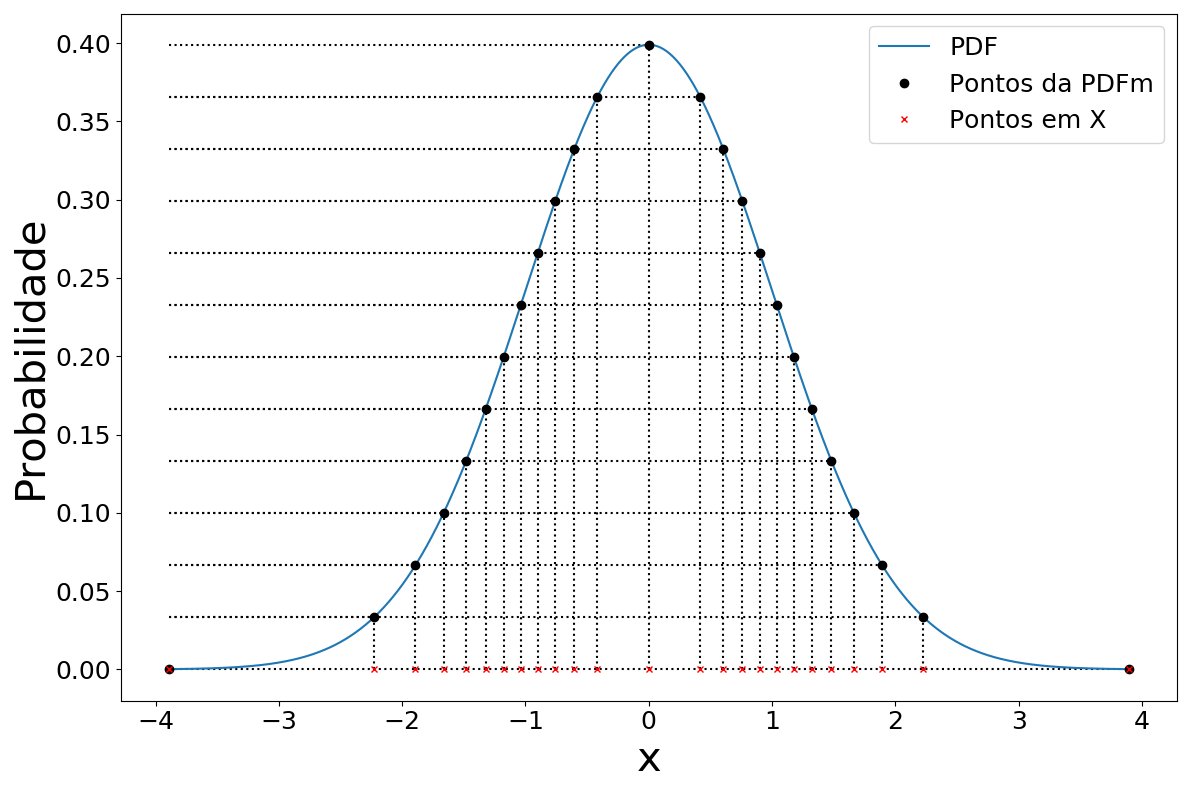
\includegraphics[width=0.67\linewidth]{./figuras/PDFm_normal_1}
	\caption{Ilustração da discretização da distribuição Gaussiana baseada em sua PDF.}
	\label{fig:PDFm_curve}
\end{figure}

Ela possui o efeito de incrementar o número de pontos estimados onde a inclinação da curva é mais acentuada.

\subsection{\textit{iPDF1}}

O método da \ac{iPDF1} reflete os valores verticais para o eixo horizontal usando a \ac{CDF} da primeira derivada da \ac{PDF} como uma transformação de base, como é ilustrado nas Figuras~\ref{fig:dPDF1} e \ref{fig:dPDF2}

\begin{figure}[!ht]
	\centering
	\begin{subfigure}[b]{0.44\textwidth}
		\centering 
		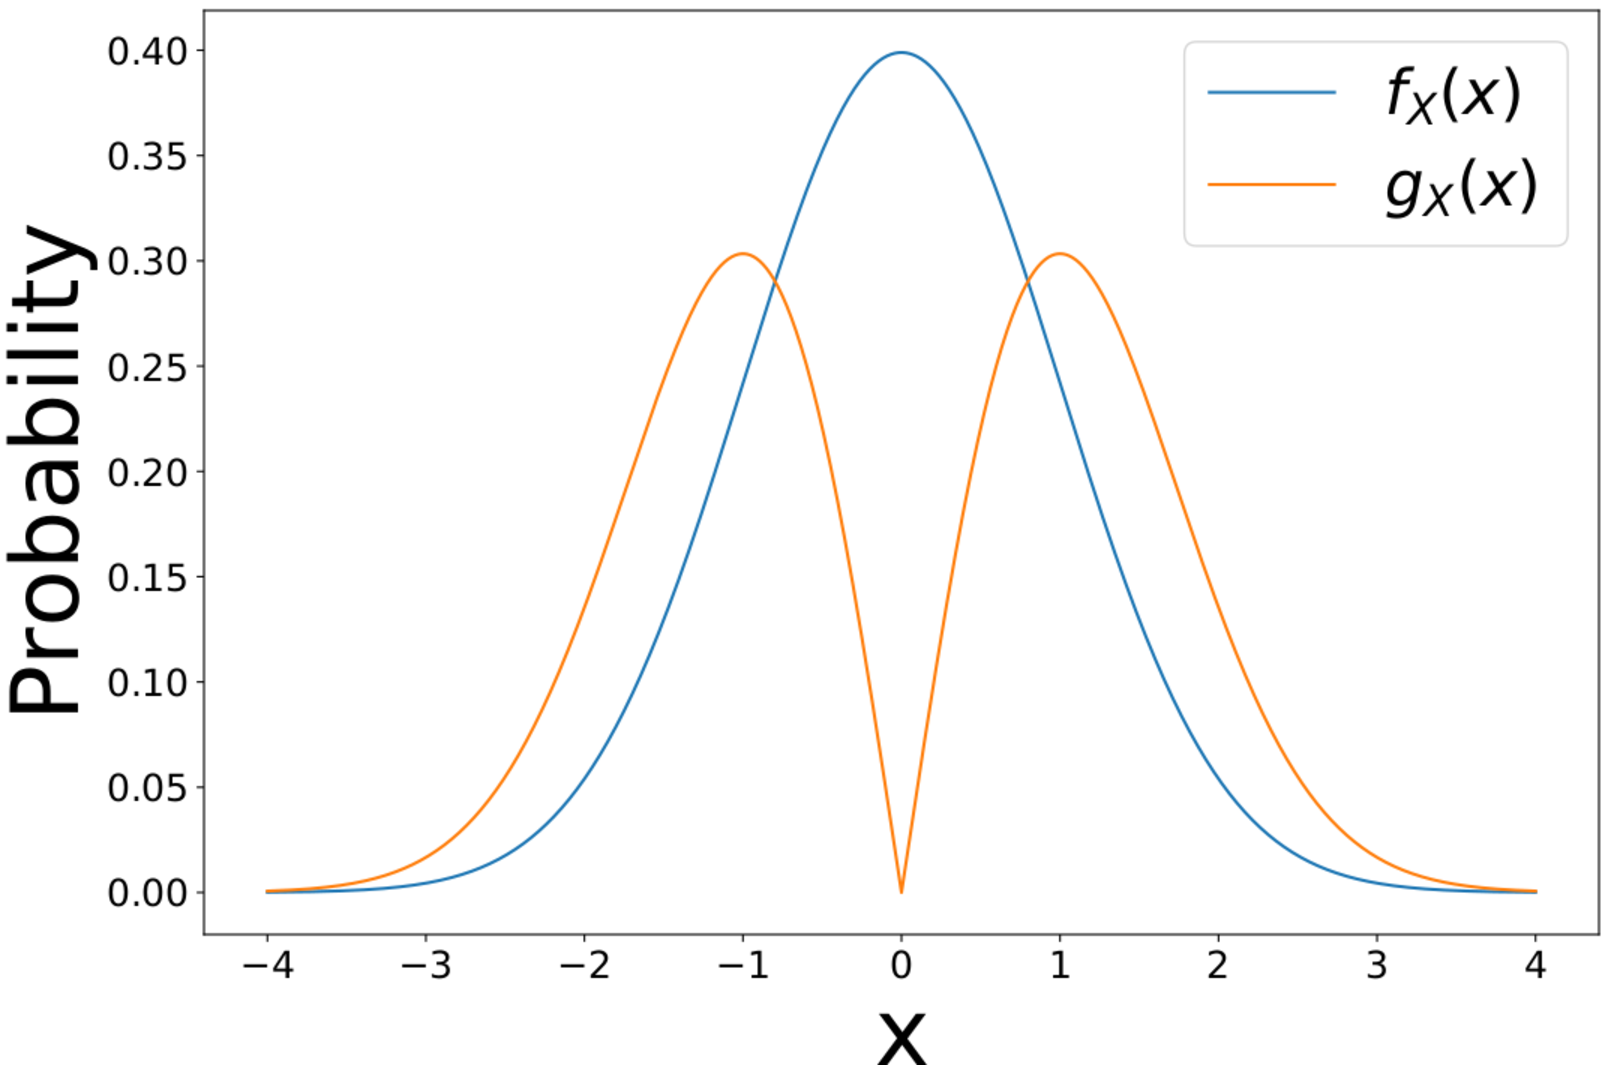
\includegraphics[width=\textwidth]{./figuras/dpdf1}
		\caption{}
		\label{fig:dPDF1}
	\end{subfigure}
	\hfill
	\begin{subfigure}[b]{0.47\textwidth}
		\centering 
		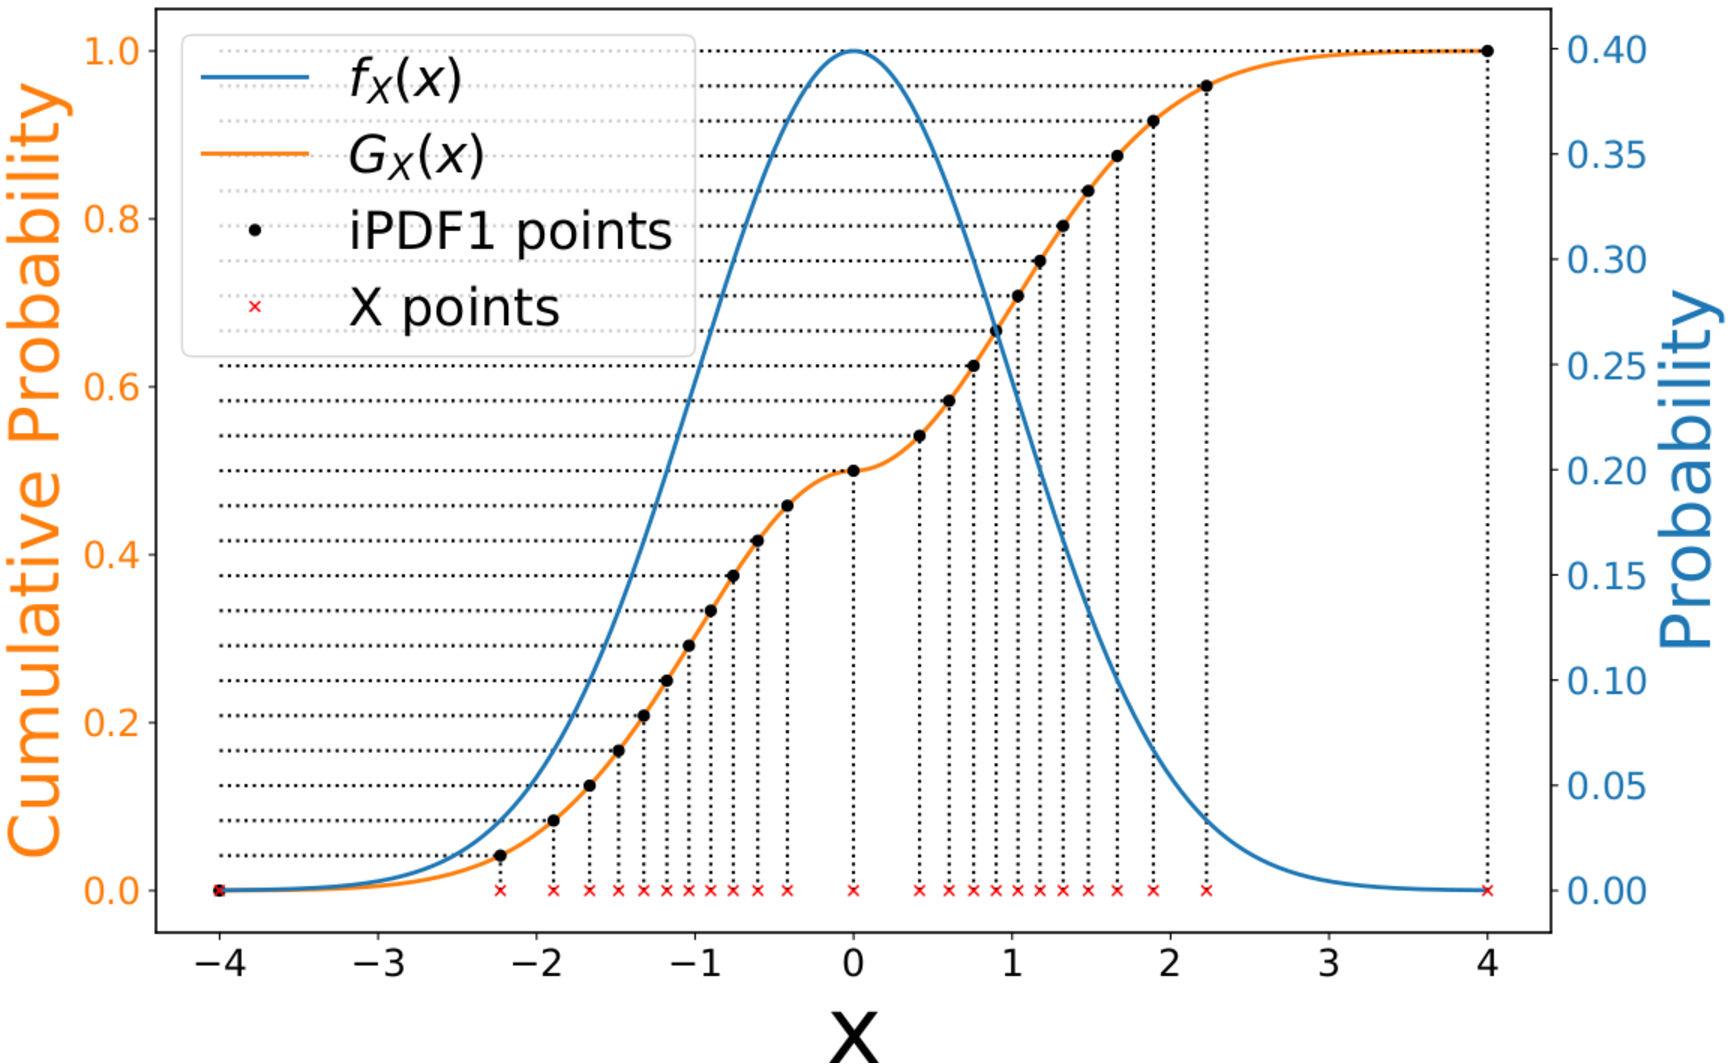
\includegraphics[width=\textwidth]{./figuras/dpdf2}
		\caption{}
		\label{fig:dPDF2}
	\end{subfigure}
	\caption{PDF Gaussiana e sua primeira derivada à esquerda. Ilustração da discretização da distribuição Gaussiana baseada na CDF da sua primeira derivada à direita.}
	\label{fig:dPDF}
\end{figure}

As equações \eqref{equ:dpdf1} e \eqref{equ:dcdf} descrevem este método matematicamente.

\begin{equation}
\begin{array}{l}
\vspace{0.3cm}\displaystyle \zeta(x) = \frac{|\mu-x|}{\sigma^3\sqrt{2\pi}}\cdot e^{\left(\frac{-(\mu-x)^2}{2\sigma^2}\right) } \\
\vspace{0.3cm} \displaystyle \int_{-\infty}^{\infty} \zeta(x)\cdot dx = c_1 \\
\displaystyle g_X(x) = \frac{\zeta(x)}{c_1}
\label{equ:dpdf1}
\end{array}
\end{equation}
onde $\zeta$ é a equação da distribuição da derivada da distribuição normal, $\mu$ é a média, $\sigma$ o desvio padrão, $x$ a variável aleatória, $c_1$ é a área abaixo da curva $\zeta$, e $g_X$ é a versão normalizada.	
A \ac{CDF} de $g_X$ ($G_X(x)$) é usada para transferir os valores da abscissa ao eixo da ordenada como mostra a  Figura~\ref{fig:dPDF2}.

\begin{equation}
G_X(x) = \int_{-\infty}^x g_X(y)\cdot dy
\label{equ:dcdf}
\end{equation}

É possível notar que este método consegue fazer uma melhor estimação nas regiões em que a primeira derivada de sua \ac{PDF} são maiores.

\subsection{\textit{iPDF2}}
Este método é construído da mesma maneira da \textit{IPDF1} mas usando a segunda derivada ao invés da primeira, como é mostrado na Figura~\ref{fig:ddPDF1} e \ref{fig:ddPDF2}. Suas equações são mostradas em \eqref{equ:hx} e \eqref{equ:ddcdf}.

\begin{figure}[ht]
	\centering
	\begin{subfigure}[b]{0.44\textwidth}
		\centering 
		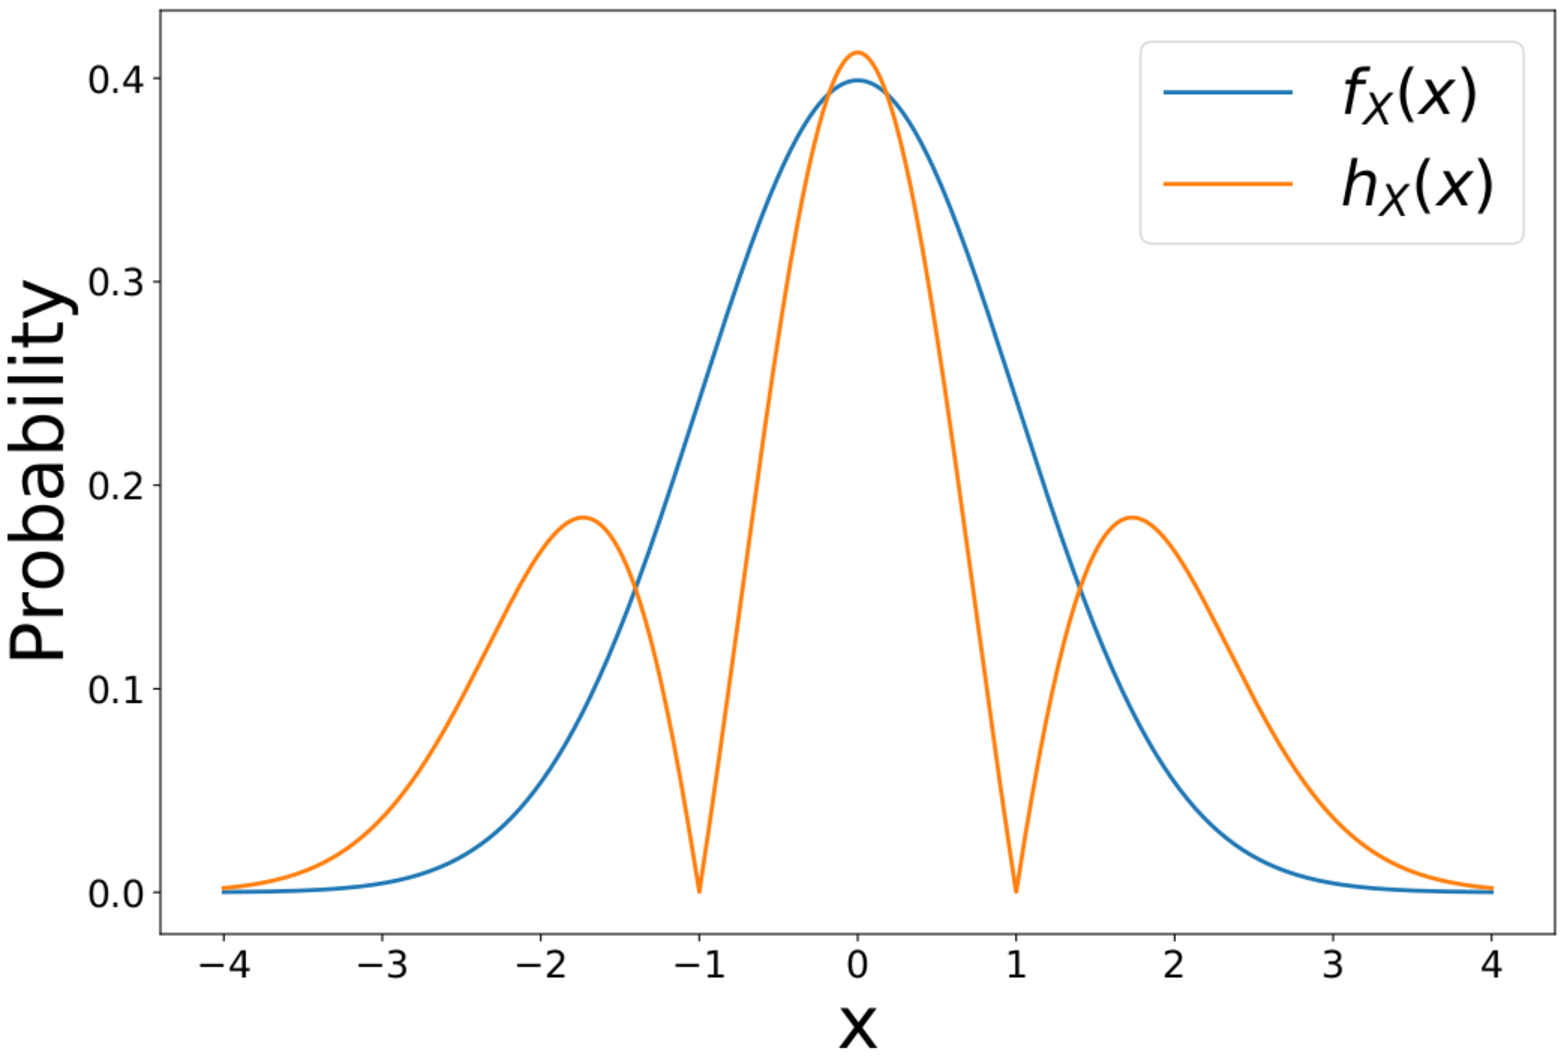
\includegraphics[width=\textwidth]{./figuras/ddpdf1.pdf}
		\caption{}
		\label{fig:ddPDF1}
	\end{subfigure}
	\hfill
	~ %add desired spacing between images, e. g. ~, \quad, \qquad, \hfill etc. 
	%(or a blank line to force the subfigure onto a new line)
	\begin{subfigure}[b]{0.47\textwidth}
		\centering 
		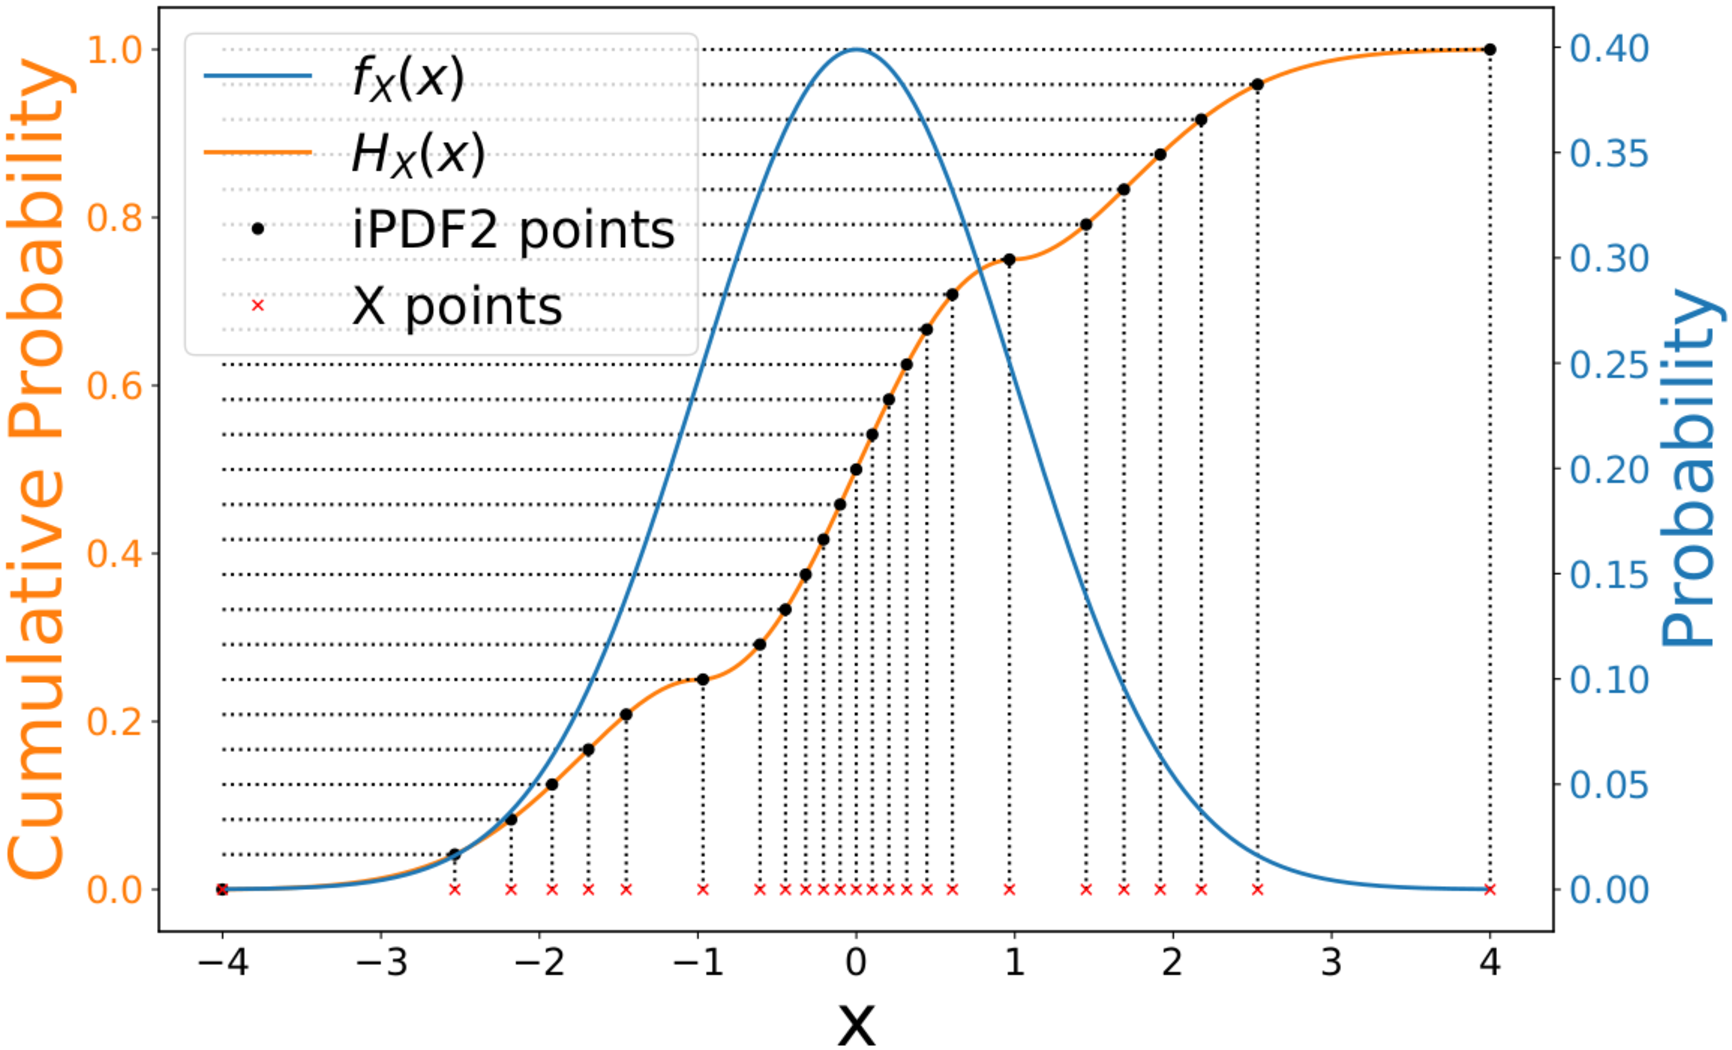
\includegraphics[width=\textwidth]{./figuras/ddpdf2.pdf}
		\caption{}
		\label{fig:ddPDF2}
	\end{subfigure}
	
	\caption{PDF Gaussiana e sua segunda derivada à esquerda. Ilustração da discretização da distribuição Gaussiana baseada na CDF da sua segunda derivada à direita.}
	\label{fig:ddPDF}
\end{figure}

\begin{equation}
\begin{array}{l}
\vspace{0.3cm}\displaystyle \eta(x) = \frac{|\sigma^2 - (\mu - x)^2|}{ \sigma^5\sqrt{2\pi}}\cdot e^{-\frac{(\mu - x)^2}{2 \sigma^2}} \\
\vspace{0.3cm} \displaystyle \int_{-\infty}^{\infty} \eta(x)\cdot dx = c_2 \\
\displaystyle h_X(x) = \frac{\eta(x)}{c_2}
\label{equ:hx}
\end{array}
\end{equation}
onde $\eta$ é a equação de distribuição de segunda derivada da distribuição Normal, $c_2$ é a área abaixo da curva desta distribuição, e $h_X$ é sua versão normalizada. 
Finalmente, $H_X(x)$ é a \ac{CDF} de $h_X$, dada por \eqref{equ:ddcdf}.

\begin{equation}
H_X(x) = \int_{-\infty}^x h_X(y)\cdot dy
\label{equ:ddcdf}
\end{equation}

Como é possível notar, há uma maior concentração de pontos onde a segunda derivada é maior.


Uma análise mais afunda sobre estes métodos será mostrada nos capítulos abaixo.
